
\documentclass[fleqn,addpoints]{exam}
\usepackage{amsmath}
\usepackage{graphicx}
\usepackage{booktabs}
\usepackage{float}
\usepackage{caption}
\usepackage{polynom}
\usepackage{mdwlist}
\usepackage{cancel}

\usepackage{unitsdef} 
\newunit{\inch}{in}
\newunit{\mile}{mile}
\newunit{\mph}{mph}
\newunit{\foot}{ft}
\newunit{\knot}{knot}
\newunit{\gallon}{gallon}

\bracketedpoints
\everymath{\displaystyle}

\printanswers

\ifprintanswers 
\usepackage{2in1, lscape} 
\fi


% \begin{figure}[H]
%   \centering
%   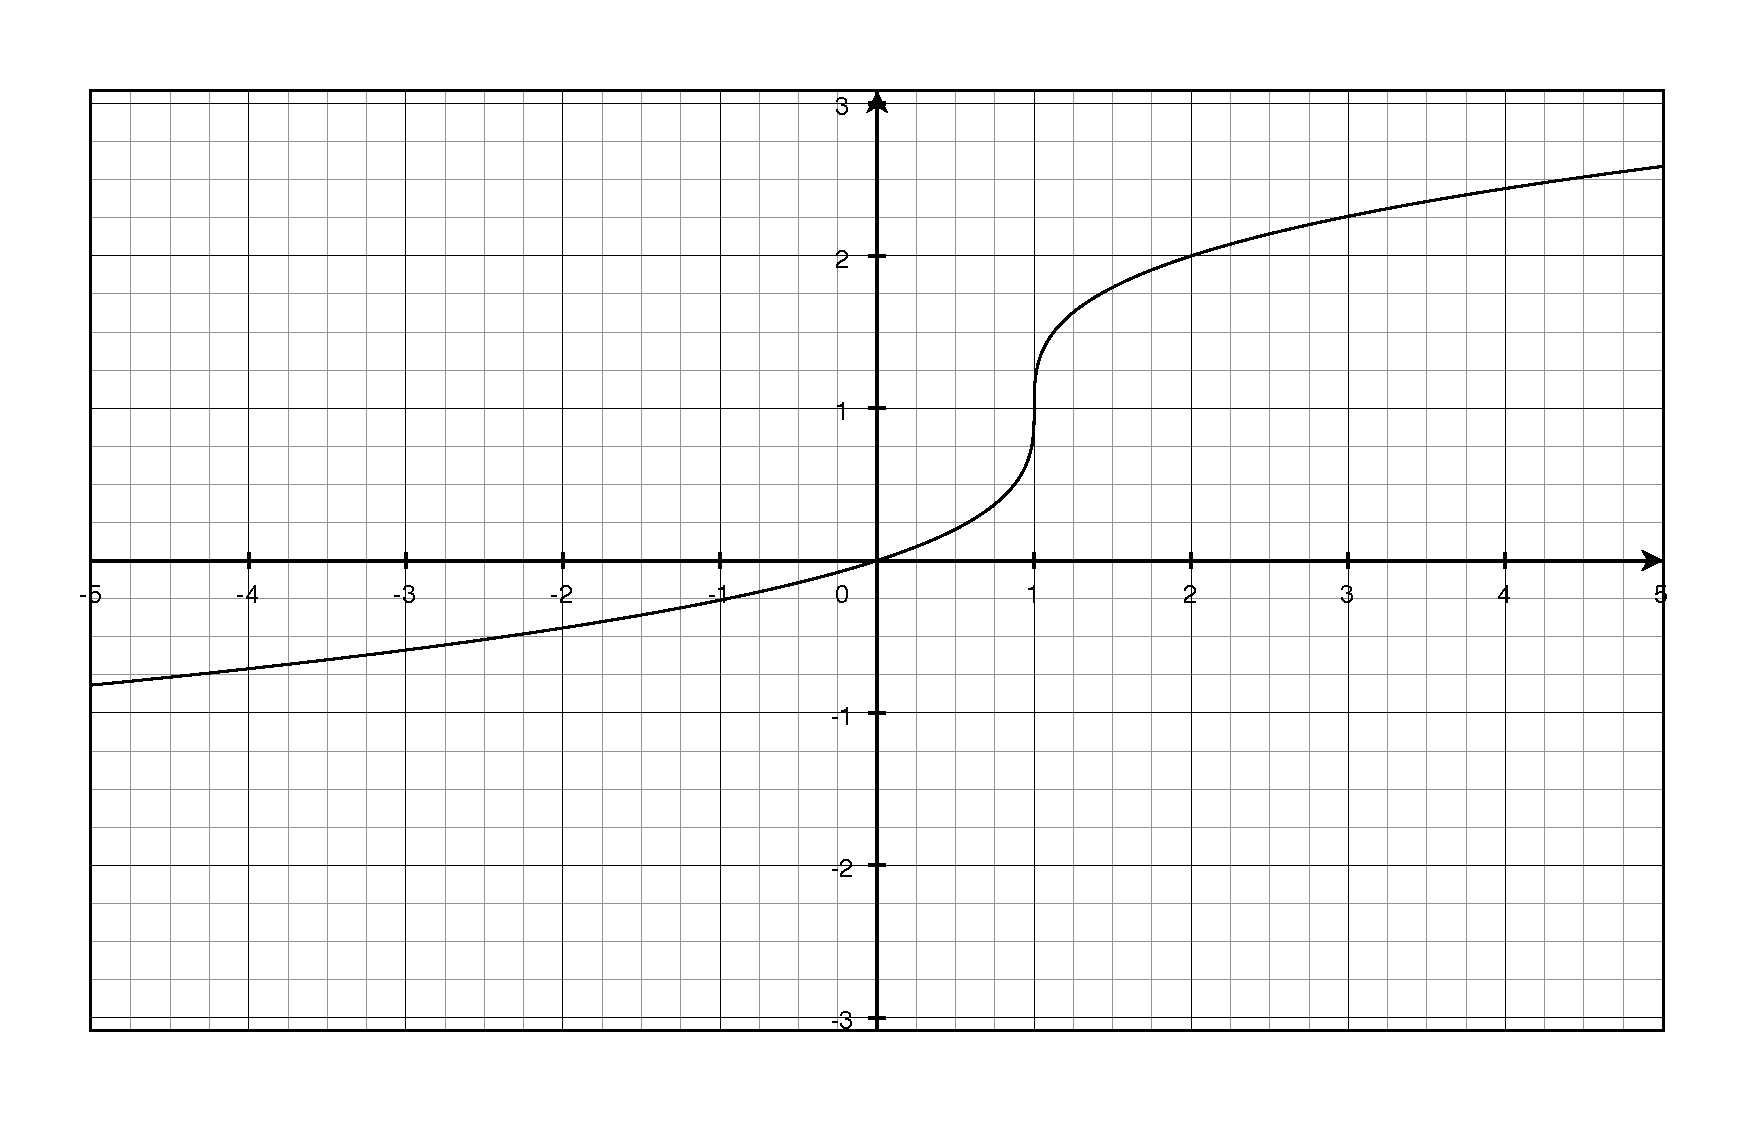
\includegraphics[scale=.3]{question7.eps}
%   \caption*{Question 7}
% \end{figure}

% \begin{tabular}{cc}
% \toprule
% period & amplitude \\
% \midrule
%   $\pi$ & $2$ \\
% \bottomrule
% \end{tabular}


%% \ifprintanswers
%% \usepackage{2in1, lscape}
%% \fi

\title{Math 263A Sample Final Three}

\date{October 25, 2012}

\author{}

\begin{document}

% from fall 2009 final

\maketitle  

\begin{questions}

\question Find the derivative of the function: $y = \frac{t^2}{3t^2 - 2t + 1}$
\begin{solution}
\begin{align*}
  y &= \frac{t^2}{3t^2 - 2t + 1} \\
  y' &= \frac{(3t^2 - 2t + 1)2t - t^2(6t - 2)}{(3t^2 - 2t + 1)^2} \\
     &= \frac{6t^3 - 4t^2 + 2t - 6t^3 + 2t^2)}{(3t^2 - 2t + 1)^2} \\
     &= \frac{- 2t^2 + 2t}{(3t^2 - 2t + 1)^2} \\
\end{align*}

\end{solution}

\question Sketch the graph of a single function $f$ for which all of the following hold:
\begin{itemize}
\item $f(2) = 1$
\item $\lim_{x \to -2} f(x) = \infty$
\item $\lim_{x \to \infty} f(x) = 3$,
\item $\lim_{x \to -\infty} f(x) = -3$,
\item $f(0)$ is undefined
\item $f$ has a  jump discontinuity at $x = 1$.
\end{itemize}

\begin{solution}
I can't get my computer to draw this graph.
\end{solution}

\question If $27 \meter^2$ of material is available to make a box with a square base and an open top, find the largest
possible volume of the box.

\begin{solution}
If $x$ is the length of a side of the base and $y$ is the height:
\begin{align*}
  V &= x^2y \\
  A &= x^2 + 4xy \\
\end{align*}

We want to optimize the volume given a fixed area, so we should solve for $y$ in the area equation:
\begin{align*}
  A &= x^2 + 4xy \\
  4xy &= A - x^2 \\
  y &= \frac{A}{4x} - \frac{x}{4}
\end{align*}

plug the result in the volume equation:
\begin{align*}
  V &= x^2 \cdot \left( \frac{A}{4x} - \frac{x}{4} \right) \\
   &= \frac{Ax}{4} - \frac{x^3}{4} \\
\end{align*}

differentiate the volume equation to find the maximum value:
\begin{align*}
  V &= \frac{Ax}{4} - \frac{x^3}{4} \\
  V' &= \frac{A}{4} - \frac{3x^2}{4} \\
\end{align*}

find the expression for the maximum:
\begin{align*}
  \frac{A}{4} - \frac{3x^2}{4} &= 0 \\
  3x^2 &= A \\
   x^2 &= \frac{A}{3} \\
   x &= \sqrt{\frac{A}{3}} \\
\end{align*}

plug in the value for the area from the equation:
\begin{align*}
  x &=  \sqrt{\frac{27}{3}} \\
    &= 3 \meter \\
\end{align*}

plug the $x$ value into the equation for $y$ to find $y$:
\begin{align*}
  y &= \frac{A}{4x} - \frac{x}{4} \\
    &= \frac{27}{12} - \frac{3}{4} \\
    &= \frac{9}{4} - \frac{3}{4} \\
    &= \frac{3}{2} \meter \\
\end{align*}

find the volume:
\begin{align*}
  V &= x^2y \\
    &= 3^2 \cdot \frac{3}{2} \\
    &= \frac{27}{2} \meter^3 \\
\end{align*}
\end{solution}

\question Find the derivative of the function using the definition of derivative. Also find the derivative of the
function using differentiation rules and compare.  
\[
  g(x) = 2x^2
\]

\begin{solution}
\begin{align*}
  g'(x) &= \lim_{h \to 0} \frac{2 (x + h)^2 - 2x^2}{h} \\
  &= \lim_{h \to 0} \frac{2 (x^2 + 2xh + h^2) - 2x^2}{h} \\
  &= \lim_{h \to 0} \frac{2x^2 + 4xh + 2h^2 - 2x^2}{h} \\
  &= \lim_{h \to 0} \frac{4xh + 2h^2}{h} \\
  &= \lim_{h \to 0} 4x + 2h \\
  &= 4x \\
\end{align*}

This is the same result you get by using differentiation rules, of course.

\end{solution}

\question
Find the area of the largest rectangle that can be inscribed in a semicircle of radius $r$.

\begin{solution}
If the semicircle is drawn with its center at the origin, the formula for the area is: $A = 2xy$.

The corners of the rectangle must be on the circle, so they must satisfy:
\begin{align*}
  x^2 + y^2 &= r^2 \\
  y &= \sqrt{r^2 - x^2}
\end{align*}

substitute the expression for $y$ into the area equation, so that the area equation only has one variable:
\[
  A = 2xy = 2x \sqrt{r^2 - x^2}
\]

differentiate $A$:
\[
  A' = 2 \sqrt{r^2 - x^2} - \frac{2x^2}{\sqrt{r^2 - x^2}} 
\]

set $A'$ equal to zero to find the maximum:
\begin{align*}
  2 \sqrt{r^2 - x^2} - \frac{2x^2}{\sqrt{r^2 - x^2}} &= 0 \\
  x &= \frac{\sqrt{2}}{2} r \\
\end{align*}

substitute back in the equation for $y$ to find $y$:
\[
  y = \sqrt{r^2 - \left( \frac{\sqrt{2}}{2} r \right)^2} = \frac{\sqrt{2}}{2} r \\
\]

The maximum area is:
\[
  A = 2 \cdot \frac{\sqrt{2}}{2} r \cdot \frac{\sqrt{2}}{2} r = r^2
\]
\end{solution}

\ifprintanswers
\pagebreak
\fi

\question Find $\frac{dy}{dx}$ using implicit differentiation: $x^2y + xy^2 = 3x$.

\begin{solution}
\begin{align*}
  x^2y + xy^2 &= 3x \\
  x^2y' + 2xy + 2xyy' + y^2 &= 3 \\
  x^2y' + 2xyy'  &= 3 - 2xy - y^2 \\
%  y'(x^2 + 2xy)  &= 3 - 2xy - y^2 \\
  y' &= \frac{3 - 2xy - y^2}{x^2 + 2xy} \\
\end{align*}

\end{solution}

\question
Find an equation of the tangent line to the curve at the given point:
\[
  y = \sin x + \cos 2x \text{, } \left( \frac{\pi}{6}, 1 \right)
\]

\begin{solution}
find the derivative:
\begin{align*}
  y  &= \sin x + \cos 2x \\
  y' &= \cos x - 2 \sin (2x) \\
\end{align*}

evaluate for $x = \frac{\pi}{6}$:
\[
  y'\left( \frac{\pi}{6} \right) = \cos \frac{\pi}{6} - 2 \sin \frac{\pi}{3} = - \frac{\sqrt{3}}{2}
\]

find the equation for the line:
\[
  y - 1 = - \frac{\sqrt{3}}{2} \left(x - \frac{\pi}{6} \right) \\
\]

\end{solution}

\ifprintanswers
\pagebreak
\fi

\question Use a linear approximation to estimate the number $(2.02)^6$.
\begin{solution}
\begin{align*}
  y &= x^6 \\
  dy &= 6x^5 \, dx \\
\\
  dy &= 6 \cdot 2^5 \cdot 0.02 \\
     &= 3.84
\\
  (2.02)^6 &\approx 2^6 + 3.84 \\
  &= 67.84 \\
\end{align*}

\end{solution}

\question Gravel is being dumped from a conveyor belt at a rate of $3 \meter^3/\minute$, and its coarseness is such
that it forms a pile in the shape of a cone whose base diameter and height are always equal. How fast is the height of
the pile increasing when the pile is $4 \meter$ high.

\begin{solution}
The volume of a cone is: $V = \frac{1}{3} \pi r^2h$

For this cone, the radius is always half the height: $r = \frac{h}{2}$.  We can plug this in to the volume equation to
get an equation that is just based on the height:
\[
  V = \frac{1}{3} \pi r^2h = \frac{\pi h^3}{12}
\] 

differentiate the volume to find the rate for the height:
\begin{align*}
  \frac{dV}{dt} &= \frac{\pi h^2}{4} \cdot \frac{dh}{dt} \\
  \frac{dh}{dt} &= \frac{4}{\pi h^2} \cdot \frac{dV}{dt} \\
\end{align*}

Plug in the values from the problem to find $\frac{dh}{dt}$:
\[
  \frac{dh}{dt} = \frac{4}{\pi 4^2} \cdot \frac{dV}{dt} = \frac{3}{4 \pi}
\]

\end{solution}

\question
The position function of a particle is given by $s = t^3 - 4t^2 - 6t$. ($s$ is given in meters and $t$ in seconds.
\begin{parts}
\part When does the particle reach a velocity of $4 \meter / \second$? 
\begin{solution}
\begin{align*}
  v &= 3t^2 - 8t - 6 \\
\\
  3t^2 - 8t - 6 &= 4 \\
  3t^2 - 8t - 10 &= 0 \\
\\
  x &= \frac{8 \pm \sqrt{64 + 4 \cdot 10 \cdot 3}}{6} \\
    &\approx 3.594 \second \\
\end{align*}

\end{solution}

\part When is the acceleration 0?
\begin{solution}
\begin{align*}
  a &= 6t - 8 \\
\\
  6t - 8 &= 0 \\
  t &= \frac{4}{3} \second \\  
\end{align*}

\end{solution}

\end{parts}

\ifprintanswers
\pagebreak
\fi

\question
Find the absolute maximum and minimum values of $f$ on the given interval. 
\[
  f(x) = \frac{x}{x^2 + 4} \text{ , } [0, 3].
\]

\begin{solution}
\begin{align*}
  f(x) &= \frac{x}{x^2 + 4} \\
  f'(x) &= \frac{(x^2 + 4) - x(2x)}{(x^2 + 4)^2} \\
        &= \frac{4 - x^2}{(x^2 + 4)^2} \\
\\
  4 - x^2 &= 0 \\
  x &= \pm 2 \\
\end{align*}

\begin{tabular}{cc}
\toprule
x & f(x) \\
\midrule
0 & 0 \\
2 & $1/4$ \\
3 & $3/13$ \\
\bottomrule
\end{tabular}

\begin{itemize*}
\item minimum: $(0, 0)$
\item maximum: $\left(2, \frac{1}{4} \right)$
\end{itemize*}

\end{solution}

\ifprintanswers
\pagebreak
\fi

\question
Find the derivative of the function $f(x) = \sin \sqrt{1 + x^2}$.

\begin{solution}
\begin{align*}
  f(x) &= \sin (1 + x^2)^{1/2} \\
  f'(x) &= \cos(1 + x^2)^{1/2} \cdot \frac{1}{2} (1 + x^2)^{-1/2} \cdot 2x \\
        &= \frac{x \cos \sqrt{1 + x^2}}{\sqrt{1 + x^2}} \\
\end{align*}
\end{solution}

\question $f(x) = 2x^3 - 3x^2 - 12x$
\begin{parts}
\part Find the intervals on which $f$ is increasing or decreasing. 
\begin{solution}
\begin{align*}
  f(x) = 2x^3 - 3x^2 - 12x \\
  f'(x) &= 6x^2 - 6x - 12 \\
\\
  6x^2 - 6x - 12 &= 0 \\
  x^2 - x - 2 &= 0 \\
  (x - 2)(x + 1) &= 0 \\
  x &= \{-1, 2\} \\
\end{align*}

\begin{itemize*}
  \item increasing: $(-\infty, -1) \cup (2, \infty)$
  \item decreasing: $(-1, 2)$
\end{itemize*}
\end{solution}

\ifprintanswers
\pagebreak
\fi

\part Find the intervals of concavity and the inflection points. 
\begin{solution}
\begin{align*}
  f'(x) &= 6x^2 - 6x - 12 \\
  f''(x) &= 12x - 6 \\
\\
  12x - 6 &= 0 \\
  12x &= 6 \\
  x &= \frac{1}{2} \\
\end{align*}

\begin{itemize*}
  \item concave down: $\left( -\infty, \frac{1}{2} \right)$
  \item concave up: $\left( \frac{1}{2}, \infty \right)$
\end{itemize*}
\end{solution}

\part Use the information from (a)-(b) to sketch the graph. 
\begin{solution}
\begin{figure}[H]
  \centering
  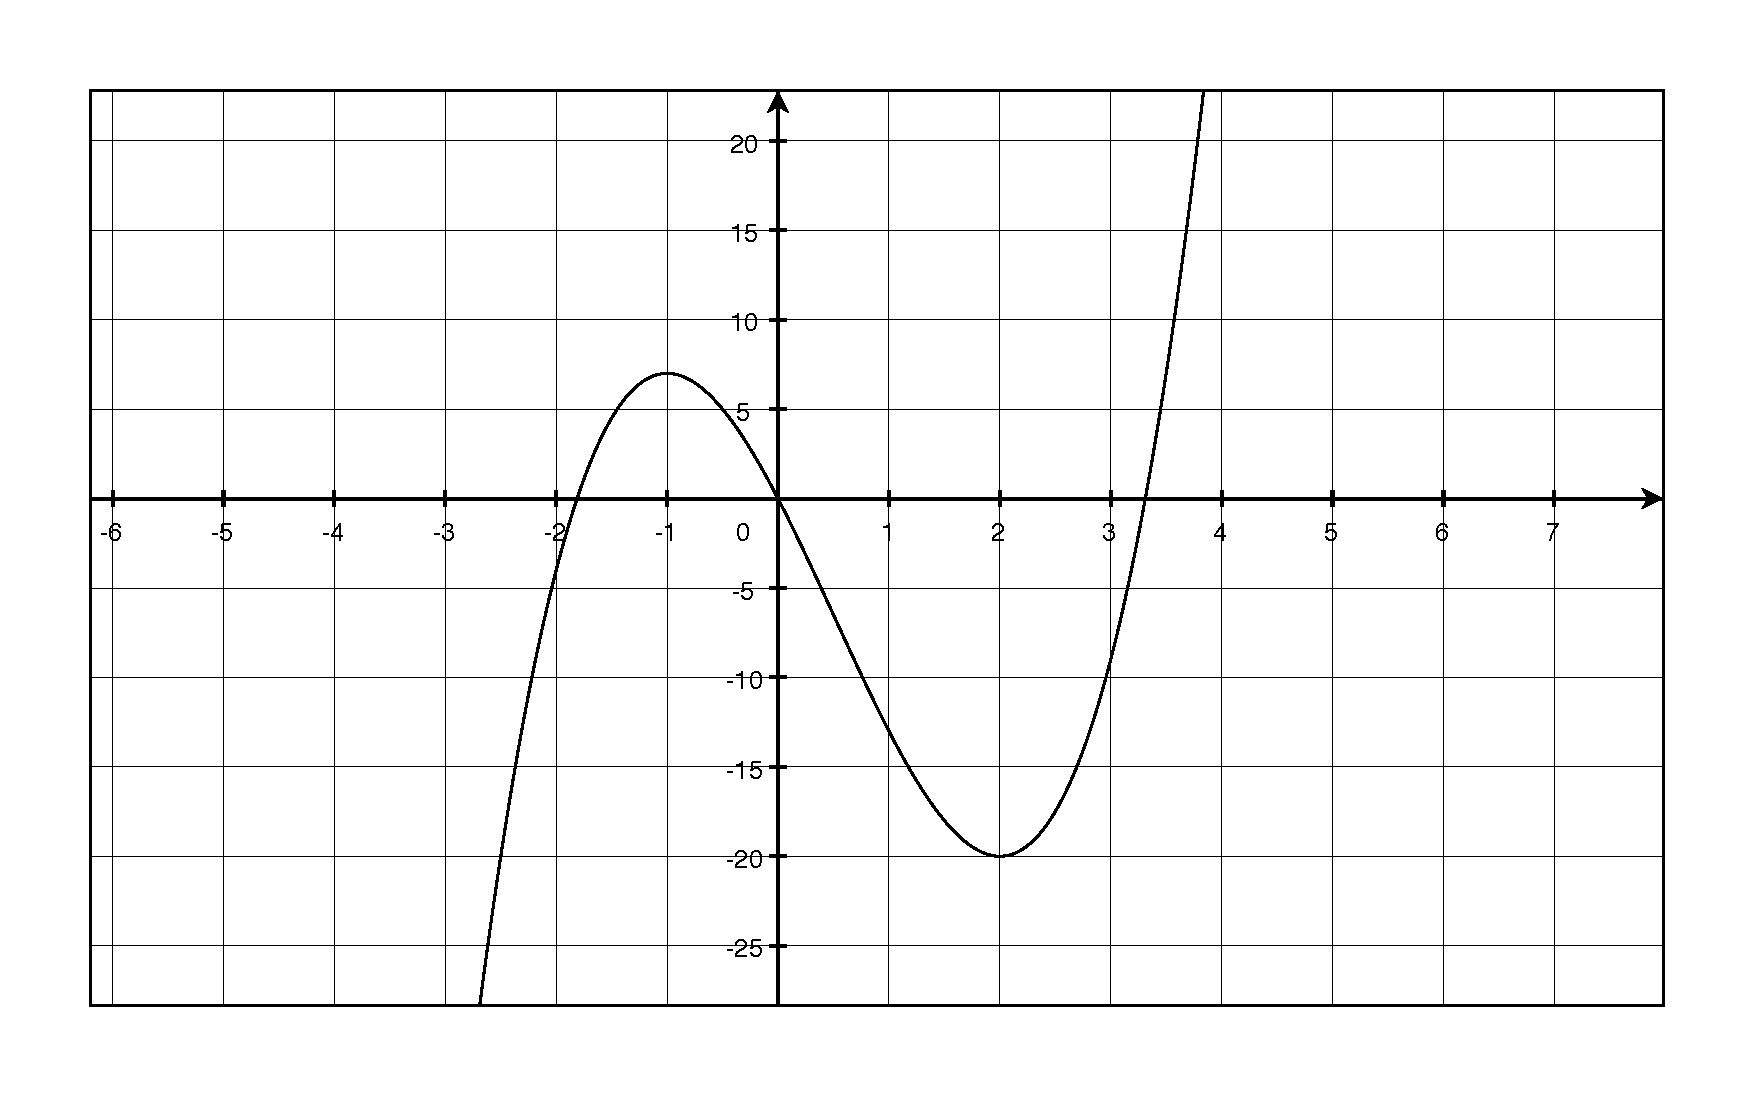
\includegraphics[scale=.3]{final_3_q13.eps}
  \caption*{Question 13}
\end{figure}
\end{solution}

\end{parts}

\question
Find the limit:
\[
  \lim_{h \to 0} \frac{\sqrt{1 + h} - 1}{h}
\]

\begin{solution}
\begin{align*}
  \lim_{h \to 0} \frac{\sqrt{1 + h} - 1}{h} &= \lim_{h \to 0} \frac{\sqrt{1 + h} - 1}{h} 
      \cdot \frac{\sqrt{1 + h} + 1}{\sqrt{1 + h} + 1} \\
  &= \lim_{h \to 0} \frac{1 + h - 1}{h (\sqrt{1 + h} + 1)} \\
  &= \lim_{h \to 0} \frac{h}{h (\sqrt{1 + h} + 1)} \\
  &= \lim_{h \to 0} \frac{1}{\sqrt{1 + h} + 1} \\
  &= \frac{1}{2} \\  
\end{align*}

\end{solution}

\question
At noon, ship A is $150 \kilometer$ west of ship B.  Ship A is sailing east at $35 \kilometer / \hour$ and ship B is
sailing north at $25 \kilometer / \hour$.  How fast is the distance between the ships changing at 4:00 PM?

\begin{solution}
The ships are sailing on the legs of a right triangle, so the distance between them is:
\[
  r^2 = x^2 + y^2
\]

differentiate to find the rates:
\begin{align*}
  r^2 &= x^2 + y^2 \\
  \frac{dr}{dt} &= \frac{x}{r} \frac{dx}{dt} + \frac{y}{r} \frac{dy}{dt}
\end{align*}

At the time we're interested in:
\begin{itemize}
\item $\frac{dx}{dt} = 35 \kilometer / \hour$
\item $\frac{dy}{dt} = 25 \kilometer / \hour$
\item $x = -10 \km$
\item $y = 100 \km$
\item $r \approx 100.5 \km$
\end{itemize}

plug all this in to get the rate the distance between the ships is changing:
\begin{align*}
  \frac{dr}{dt} &= \frac{x}{r} \frac{dx}{dt} + \frac{y}{r} \frac{dy}{dt}  \\
     &= \frac{-10}{100.5} \cdot 35 + \frac{100}{100.5} \cdot 25 \\
     &\approx 21.4 \kilometer / \hour \\
\end{align*}

\end{solution}

\end{questions}

\end{document}
